\documentclass[10pt]{article}

\usepackage[utf8]{inputenc}
\usepackage[spanish]{babel}
\decimalpoint
\usepackage{amsmath, amssymb}
\usepackage{xcolor}
\usepackage{geometry}
\geometry{letterpaper, margin=1in}
\usepackage{graphicx}
\usepackage{hyperref}
\usepackage{float}
\usepackage{colortbl}
\usepackage{caption}
%%%%%%%%%%%%%%%%%%%%%%%%%%%%%%%%%%%%%%%%%%%%%%%%%%%%%%%%%%%%%%%%%%%%%%%%%%%%%%%%%%%%%%%%%%%%%%%%%%%%%%%%%%%%%%%%%%%%%%%%%%%%%%%%%%%%%%%%%%%%%%%%%%%%%%%%%%%%%%%%%%%%%%%%%%%%%%%%%%%%%%%%%%%%%%
%%%%%%%%%%%%%%%%%%%%%%%%%%%%%%%%%%%%%%%%%%%%%%%%%%%%%%%%%%%%%%%%%%%%%%%%%%%%%%%%%%%%%%%%%%%%%%%%%%%%%%%%%%%%%%%%%%%%%%%%%%%%%%%%%%%%%%%%%%%%%%%%%%%%%%%%%%%%%%%%%%%%%%%%%%%%%%%%%%%%%%%%%%%%%%
\title{Universidad Panamericana \\ Maestría en Ciencia de Datos 
\\ Econometría \\ \vspace{0.5cm} Actividad Desestacionalización de Series de Tiempo}

\author{Enrique Ulises Báez Gómez Tagle\\Luis Alejandro Guillén Alvarez}

\date{\today}
%%%%%%%%%%%%%%%%%%%%%%%%%%%%%%%%%%%%%%%%%%%%%%%%%%%%%%%%%%%%%%%%%%%%%%%%%%%%%%%%%%%%%%%%%%%%%%%%%%%%%%%%%%%%%%%%%%%%%%%%%%%%%%%%%%%%%%%%%%%%%%%%%%%%%%%%%%%%%%%%%%%%%%%%%%%%%%%%%%%%%%%%%%%%%%
%%%%%%%%%%%%%%%%%%%%%%%%%%%%%%%%%%%%%%%%%%%%%%%%%%%%%%%%%%%%%%%%%%%%%%%%%%%%%%%%%%%%%%%%%%%%%%%%%%%%%%%%%%%%%%%%%%%%%%%%%%%%%%%%%%%%%%%%%%%%%%%%%%%%%%%%%%%%%%%%%%%%%%%%%%%%%%%%%%%%%%%%%%%%%%
\begin{document}

\maketitle

\tableofcontents

\newpage
%%%%%%%%%%%%%%%%%%%%%%%%%%%%%%%%%%%%%%%%%%%%%%%%%%%%%%%%%%%%%%%%%%%%%%%%%%%%%%%%%%%%%%%%%%%%%%%%%%%%%%%%%%%%%%%%%%%%%%%%%%%%%%%%%%%%%%%%%%%%%%%%%%%%%%%%%%%%%%%%%%%%%%%%%%%%%%%%%%%%%%%%%%%%%%
%%%%%%%%%%%%%%%%%%%%%%%%%%%%%%%%%%%%%%%%%%%%%%%%%%%%%%%%%%%%%%%%%%%%%%%%%%%%%%%%%%%%%%%%%%%%%%%%%%%%%%%%%%%%%%%%%%%%%%%%%%%%%%%%%%%%%%%%%%%%%%%%%%%%%%%%%%%%%%%%%%%%%%%%%%%%%%%%%%%%%%%%%%%%%%
\section{Contexto}
  México es el mayor productor y exportador mundial de aguacate, una fruta que ha ganado popularidad global 
  por su valor nutricional y versatilidad en la cocina. El aguacate, conocido por su riqueza en grasas 
  saludables, vitaminas y minerales, es un componente esencial en dietas equilibradas y ha visto un aumento 
  significativo en su demanda en mercados internacionales.

  La industria del aguacate es un pilar fundamental de la economía agrícola mexicana. En las últimas 
  décadas, el aguacate ha pasado de ser un producto regional a convertirse en una de las principales 
  exportaciones agrícolas del país. La producción y exportación de aguacate no solo contribuyen de manera 
  significativa al PIB agrícola, sino que también generan empleo en diversas regiones, particularmente en 
  los estados de Michoacán y Jalisco, que son los principales productores.

  A continuación en la tabla no1 se muestran los datos bimestrales de la exportación de aguacate en toneladas:
%%%%%%%%%%%%%%%%%%%%%%%%%%%%%%%%%%%%%%%%%%%%%%%%%%%%%%%%%%%%%%%%%%%%%%%%%%%%%%%%%%%%%%%%%%%%%%%%%%%%%%%%%%%%%%%%%%%%%%%%%%%%%%%%%%%%%%%%%%%%%%%%%%%%%%%%%%%%%%%%%%%%%%%%%%%%%%%%%%%%%%%%%%%%%%
\begin{table}[H]
  \centering
  \caption{Exportación bimestral de aguacate (toneladas)}
  \label{tab:export_avocado}
  \begin{tabular}{l c c r}
  \hline
  \textbf{Año} & \textbf{Bimestre} & \textbf{t} & \textbf{Toneladas} \\
  \hline
    2019 & 1 & 1  & 224,604.04 \\
    2019 & 2 & 2  & 201,125.90 \\
    2019 & 3 & 3  & 154,184.06 \\
    2019 & 4 & 4  & 140,857.77 \\
    2019 & 5 & 5  & 213,070.50 \\
    2019 & 6 & 6  & 268,644.20 \\
    2020 & 1 & 7  & 316,793.52 \\
    2020 & 2 & 8  & 283,659.09 \\
    2020 & 3 & 9  & 217,428.69 \\
    2020 & 4 & 10 & 198,535.98 \\
    2020 & 5 & 11 & 300,467.80 \\
    2020 & 6 & 12 & 378,764.26 \\
    2021 & 1 & 13 & 410,806.71 \\
    2021 & 2 & 14 & 367,955.31 \\
    2021 & 3 & 15 & 282,092.18 \\
    2021 & 4 & 16 & 257,532.45 \\
    2021 & 5 & 17 & 389,706.87 \\
    2021 & 6 & 18 & 491,240.80 \\
    2022 & 1 & 19 & 405,077.56 \\
    2022 & 2 & 20 & 362,765.23 \\
    2022 & 3 & 21 & 278,092.64 \\
    2022 & 4 & 22 & 253,986.68 \\
    2022 & 5 & 23 & 384,156.60 \\
    2022 & 6 & 24 & 484,431.36 \\
    2023 & 1 & 25 & 426,151.46 \\
    2023 & 2 & 26 & 381,653.51 \\
    2023 & 3 & 27 & 292,635.95 \\
    2023 & 4 & 28 & 267,180.48 \\
    2023 & 5 & 29 & 404,208.92 \\
    2023 & 6 & 30 & 522,430.98 \\
  \hline
  \end{tabular}
\end{table}
%%%%%%%%%%%%%%%%%%%%%%%%%%%%%%%%%%%%%%%%%%%%%%%%%%%%%%%%%%%%%%%%%%%%%%%%%%%%%%%%%%%%%%%%%%%%%%%%%%%%%%%%%%%%%%%%%%%%%%%%%%%%%%%%%%%%%%%%%%%%%%%%%%%%%%%%%%%%%%%%%%%%%%%%%%%%%%%%%%%%%%%%%%%%%%
%%%%%%%%%%%%%%%%%%%%%%%%%%%%%%%%%%%%%%%%%%%%%%%%%%%%%%%%%%%%%%%%%%%%%%%%%%%%%%%%%%%%%%%%%%%%%%%%%%%%%%%%%%%%%%%%%%%%%%%%%%%%%%%%%%%%%%%%%%%%%%%%%%%%%%%%%%%%%%%%%%%%%%%%%%%%%%%%%%%%%%%%%%%%%%
\section{Preguntas}
\begin{enumerate}
    \item Si establecemos como “regla de dedo” que una serie presenta poca variación si el coeficiente de variación es menor a 30\%. En el caso de las exportaciones de aguacate ¿cuánto vale el coeficiente de variación? Exprese su resultado en porcentaje con dos decimales.\\
      \textcolor{blue}{
        \noindent\textbf{Coeficiente de variación (CV)} cuantifica la dispersión relativa de una variable:
        \begin{equation}
          \mathrm{CV} = \frac{s}{\bar{x}}\times 100\%,
        \end{equation}
        \noindent Obtenemos
        \begin{align}
          \bar{x} &= 318\,674.72 \,\text{toneladas},\\
          s &= 100\,061.44 \,\text{toneladas}.
        \end{align}
        Sustituyendo,
        \begin{equation}
            \mathrm{CV} = \frac{100\,061.44}{318\,674.72}\times 100\% = \mathbf{31.40\%}.
        \end{equation}
        \noindent Usando la regla de que una serie presenta poca variación si $\mathrm{CV}<30\%$, el valor obtenido de $31.40\%$ indica que las exportaciones \emph{sí muestran} una variación relativa considerable-
      }
%%%%%%%%%%%%%%%%%%%%%%%%%%%%%%%%%%%%%%%%%%%%%%%%%%%%%%%%%%%%%%%%%%%%%%%%%%%%%%%%%%%%%%%%%%%%%%%%%%%%%%%%%%%%%%%%%%%%%%%%%%%%%%%%%%%%%%%%%%%%%%%%%%%%%%%%%%%%%%%%%%%%%%%%%%%%%%%%%%%%%%%%%%%%%%
    \item Considerando las estadísticas descriptivas de la serie de tiempo de las exportaciones de aguacate ¿qué puede concluir? Incluya los gráficos relevantes para su análisis.\\
    \textcolor{blue}{
      \noindent Para la variable exportaciones de aguacate (en toneladas) se calcularon las medidas básicas de tendencia central y dispersión:
      \begin{align}
        n &= 30, \quad \text{número de observaciones},\\
        \bar{x} &= 318\,674.72 \,\text{toneladas},\\
        s &= 100\,061.44 \,\text{toneladas},\\
        \min(x) &= 140\,857.77, \quad \max(x) = 522\,430.98,\\
        Q_1 &= 254\,873.12, \quad Q_2 = 296\,551.88, \quad Q_3 = 388\,319.30.
      \end{align}
      \noindent La media se ubica en torno a 318 mil toneladas, con una desviación estándar considerable de 100 mil, lo que indica una alta variabilidad. El rango intercuartílico nos muestra que el 50\% central de los datos se concentra entre aproximadamente 255 mil y 388 mil toneladas, mientras que tenemos valores extremos que alcanzan mínimos cercanos a 141 mil y máximos de más de 522 mil toneladas.\\
      La Figura~\ref{fig:serie_bimestral} muestra la serie bimestral; la Figura~\ref{fig:hist_export} presenta la distribución de las exportaciones; la Figura~\ref{fig:box_export} muestra el boxplot de las exportaciones.
        \begin{figure}[H]
          \centering
          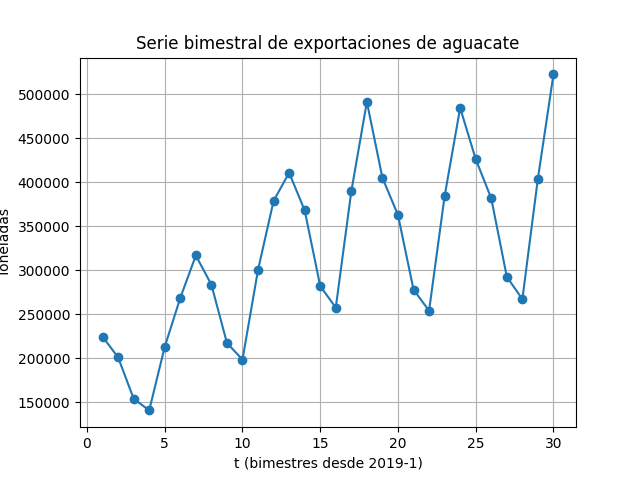
\includegraphics[width=0.65\linewidth]{../plots/python/avocado_exports_bimestral.png}
          \caption{Serie bimestral de exportaciones de aguacate (toneladas).}
          \label{fig:serie_bimestral}
        \end{figure}
        \begin{figure}[H]
            \centering
            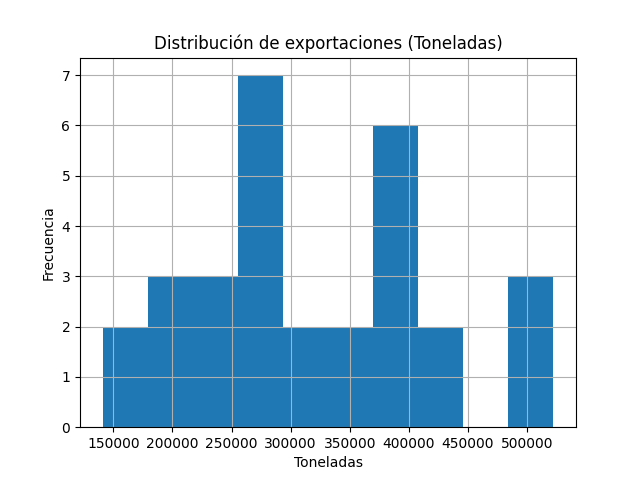
\includegraphics[width=0.80\linewidth]{../plots/python/avocado_exports_histogram.png}
            \caption{Histograma de exportaciones bimestrales (toneladas).}
            \label{fig:hist_export}
        \end{figure}
        \begin{figure}[H]
          \centering
          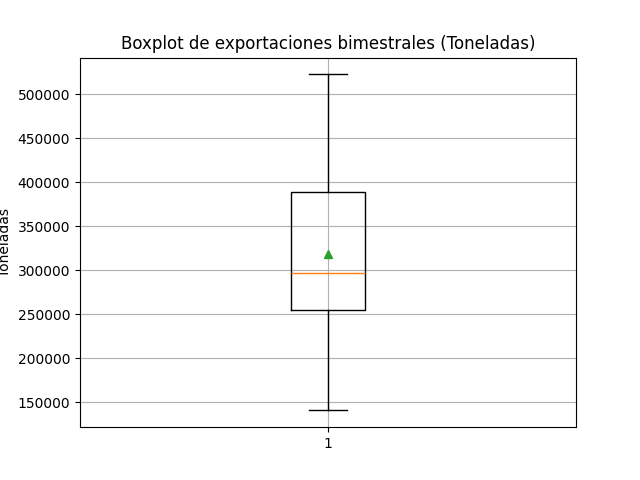
\includegraphics[width=0.80\linewidth]{../plots/python/avocado_exports_boxplot.png}
          \caption{Boxplot de exportaciones bimestrales de aguacate (toneladas).}
          \label{fig:box_export}
        \end{figure}
    }
%%%%%%%%%%%%%%%%%%%%%%%%%%%%%%%%%%%%%%%%%%%%%%%%%%%%%%%%%%%%%%%%%%%%%%%%%%%%%%%%%%%%%%%%%%%%%%%%%%%%%%%%%%%%%%%%%%%%%%%%%%%%%%%%%%%%%%%%%%%%%%%%%%%%%%%%%%%%%%%%%%%%%%%%%%%%%%%%%%%%%%%%%%%%%%
    \item Considerando un modelo de regresión de la serie original contra el tiempo, el valor del coeficiente de pendiente muestral es en miles de toneladas es:\\
    \textcolor{blue}{
      \begin{equation}
        y_t = \beta_0 + \beta_1 t + \varepsilon_t,
      \end{equation}
      donde $y_t$ representa las exportaciones (en toneladas) en el bimestre $t$, $\beta_0$ es la ordenada al origen, $\beta_1$ la pendiente que mide el cambio esperado en toneladas por cada bimestre y $\varepsilon_t$ el término de error.
      \noindent A partir de la regresión con Mínimos Cuadrados Ordinarios (MCO) se obtuvo:
      \begin{align}
        \hat{\beta}_0 &= 201{,}900 \, \text{toneladas (aprox.)},\\
        \hat{\beta}_1 &= 7{,}533.78 \, \text{toneladas/bimestre}.
      \end{align}
      \noindent En términos de miles de toneladas:
      \begin{equation}
        \hat{\beta}_1 \approx \mathbf{7.53 \,\text{mil toneladas/bimestre}}.
      \end{equation}
      \noindent La pendiente positiva indica que, en promedio, las exportaciones de aguacate han aumentado en alrededor de 7.5 mil toneladas por cada bimestre a lo largo del periodo 2019--2023.\\
    }
%%%%%%%%%%%%%%%%%%%%%%%%%%%%%%%%%%%%%%%%%%%%%%%%%%%%%%%%%%%%%%%%%%%%%%%%%%%%%%%%%%%%%%%%%%%%%%%%%%%%%%%%%%%%%%%%%%%%%%%%%%%%%%%%%%%%%%%%%%%%%%%%%%%%%%%%%%%%%%%%%%%%%%%%%%%%%%%%%%%%%%%%%%%%%%
    \item Elabore la prueba de hipótesis correspondiente con un 0.05 de significancia para validar si las exportaciones de aguacate han venido creciendo en el tiempo.\\
    \textcolor{blue}{
      \noindent Consideremos:
      \begin{align}
        H_0 &: \beta_1 \leq 0 \quad \text{(no existe tendencia creciente)}, \\
        H_1 &: \beta_1 > 0 \quad \text{(existe tendencia creciente)}.
      \end{align}
      \noindent A partir de la regresión lineal sobre la serie original se obtuvo:
      \begin{equation}
        t = \frac{\hat{\beta}_1}{\text{EE}(\hat{\beta}_1)} = \frac{7533.78}{1608.38} \approx 4.684.
      \end{equation}
      \noindent El valor $p$ bilateral reportado fue $6.58 \times 10^{-5}$, lo que implica un $p$ unilateral de:
      \begin{equation}
        p \approx 3.29 \times 10^{-5}.
      \end{equation}
      \noindent Como $p < 0.05$, se \textbf{rechaza la hipótesis nula}. Hay evidencia estadísticamente significativa para concluir que la pendiente es positiva.
      \noindent Las exportaciones de aguacate presentan una tendencia creciente en el periodo analizado.
    }
%%%%%%%%%%%%%%%%%%%%%%%%%%%%%%%%%%%%%%%%%%%%%%%%%%%%%%%%%%%%%%%%%%%%%%%%%%%%%%%%%%%%%%%%%%%%%%%%%%%%%%%%%%%%%%%%%%%%%%%%%%%%%%%%%%%%%%%%%%%%%%%%%%%%%%%%%%%%%%%%%%%%%%%%%%%%%%%%%%%%%%%%%%%%%%
    \item Aplicando la técnica de desestacionalidad simple vista en clase, obtenga los índices estacionales e intérpretelos.\\
    \textcolor{blue}{
      \noindent Para identificar la estacionalidad se calcularon índices multiplicativos por bimestre mediante:
      \begin{equation}
        I_j = \frac{\overline{y}_j}{\overline{y}},
      \end{equation}
      donde $\overline{y}_j$ es el promedio de las exportaciones en el bimestre $j$ a lo largo de los años, y $\overline{y}$ es el promedio global de toda la serie.\\
      \noindent\textbf{Resultados obtenidos:}
      \begin{align}
        I_1 &= 1.1193, & I_2 &= 1.0024, & I_3 &= 0.7685, \\
        I_4 &= 0.7017, & I_5 &= 1.0617, & I_6 &= 1.3465.
      \end{align}
      \noindent\textbf{Interpretación.} 
      \begin{itemize}
        \item Valores $I_j > 1$ indican bimestres con exportaciones por encima del promedio general.
        \item Valores $I_j < 1$ reflejan bimestres con exportaciones por debajo del promedio.
      \end{itemize}
      Particularmente
      \begin{itemize}
        \item El bimestre 6 (jul-ago) destaca con un índice de 1.3465, lo que significa un 34.7\% por encima del promedio.
        \item El bimestre 4 (may-jun) es el más bajo, con 0.7017, es decir, un 29.8\% por debajo del promedio.
        \item Los bimestres 1 y 5 también muestran exportaciones superiores al promedio, mientras que bimestres 3 y 4 son consistentemente más bajos.
      \end{itemize}
  }
  \begin{figure}[H]
    \centering
    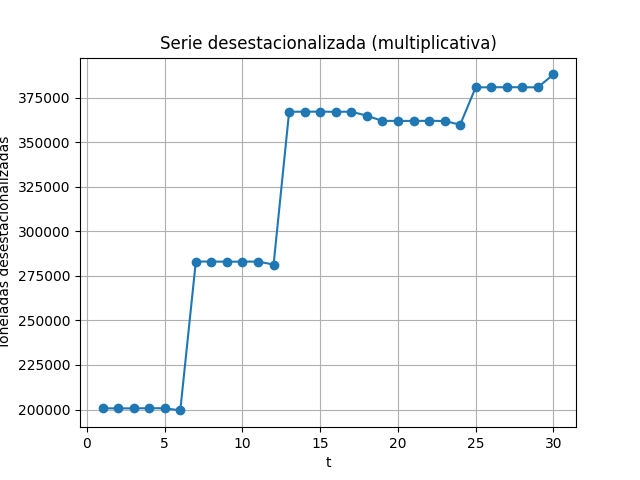
\includegraphics[width=0.80\linewidth]{../plots/python/avocado_exports_deseasonalized.png}
    \caption{Serie bimestral de exportaciones de aguacate (toneladas) desestacionalizada.}
    \label{fig:serie_bimestral_deseasonalized}
  \end{figure}
%%%%%%%%%%%%%%%%%%%%%%%%%%%%%%%%%%%%%%%%%%%%%%%%%%%%%%%%%%%%%%%%%%%%%%%%%%%%%%%%%%%%%%%%%%%%%%%%%%%%%%%%%%%%%%%%%%%%%%%%%%%%%%%%%%%%%%%%%%%%%%%%%%%%%%%%%%%%%%%%%%%%%%%%%%%%%%%%%%%%%%%%%%%%%%
    \item Obtenga la regresión lineal simple con los datos desestacionalizados y el tiempo y elabore la prueba de hipótesis correspondiente con un 0.05 de significancia para validar si la tendencia de las exportaciones de aguacate ha venido creciendo en el tiempo.\\
    \textcolor{blue}{
      \noindent Una vez que eliminamos el componente estacional, se ajusta nuevamente una regresión lineal simple:
      \begin{equation}
        y^{*}_t = \beta_0 + \beta_1 t + \varepsilon_t,
      \end{equation}
      \noindent Con Mínimos Cuadrados Ordinarios se obtuvo:
      \begin{align}
        \hat{\beta}_0 &= 209{,}000 \,\text{toneladas (aprox.)}, \\
        \hat{\beta}_1 &= 7{,}076.68 \,\text{toneladas/bimestre}.
      \end{align}
      \noindent\textbf{Prueba de hipótesis.} 
      \begin{align}
        H_0 &: \beta_1 \leq 0, \\
        H_1 &: \beta_1 > 0.
      \end{align}
      El estadístico $t$ calculado fue:
      \begin{equation}
        t = \frac{7076.68}{666.67} \approx 10.615.
      \end{equation}
      El valor-$p$ unilateral fue de $1.27 \times 10^{-11}$.\\
      Dado que $p < 0.05$, se \textbf{rechaza $H_0$}. Hay evidencia estadísticamente significativa de que la pendiente es positiva.
      Aún eliminada la estacionalidad, la tendencia de las exportaciones de aguacate sigue siendo creciente, con un incremento promedio de alrededor de 7.1 mil toneladas por bimestre.
    }
%%%%%%%%%%%%%%%%%%%%%%%%%%%%%%%%%%%%%%%%%%%%%%%%%%%%%%%%%%%%%%%%%%%%%%%%%%%%%%%%%%%%%%%%%%%%%%%%%%%%%%%%%%%%%%%%%%%%%%%%%%%%%%%%%%%%%%%%%%%%%%%%%%%%%%%%%%%%%%%%%%%%%%%%%%%%%%%%%%%%%%%%%%%%%%
    \item Proporcione un intervalo al 95\% de confianza para el valor de la tendencia de la serie de exportaciones de aguacate en el segundo bimestre del 2024.\\
    \textcolor{blue}{
      \noindent Usando el modelo de regresión de la serie original
      \begin{equation}
        y_t = \beta_0 + \beta_1 t + \varepsilon_t, \quad t=1,\dots,30,
      \end{equation}
      estimamos la media esperada (tendencia) para $t=32$ (bimestre 2 de 2024) mediante
      \begin{equation}
        \hat{y}_{32} = \hat{\beta}_0 + \hat{\beta}_1\,32.
      \end{equation}
      \noindent El intervalo de confianza al 95\% para la media condicional en $t=32$ es
      \begin{equation}
        \hat{y}_{32} \pm t_{\alpha/2,\,n-2}\;\mathrm{EE}\big(\hat{y}_{32}\big),
      \end{equation}
      donde $\mathrm{EE}(\hat{y}_{32})$ es el error estándar de la media pronosticada. Numéricamente se obtuvo
      \begin{equation}
        \boxed{\;[381\,595.30,\; 504\,368.80]\ \text{toneladas}\;}, \qquad \hat{y}_{32}=\mathbf{442\,982.05}.
      \end{equation}
      \noindent El siguiente intervalo de predicción al 95\% incorpora la variabilidad del error idiosincrático y es más amplio:
      \begin{equation}
        \hat{y}_{32} \pm t_{\alpha/2,\,n-2}\;\sqrt{\mathrm{EE}\big(\hat{y}_{32}\big)^2 + \hat{\sigma}^2}.
      \end{equation}
      En este caso:
      \begin{equation}
        \boxed{\;[275\,161.00,\; 610\,803.10]\ \text{toneladas}\;}. 
      \end{equation}
      \noindent La media esperada de la tendencia para 2024-bimestre 2 es aproximadamente 443 mil toneladas; un valor observado individual podría caer, con 95\% de confianza, dentro del intervalo de predicción indicado, que es más amplio por incluir la incertidumbre del término de error.
    }
%%%%%%%%%%%%%%%%%%%%%%%%%%%%%%%%%%%%%%%%%%%%%%%%%%%%%%%%%%%%%%%%%%%%%%%%%%%%%%%%%%%%%%%%%%%%%%%%%%%%%%%%%%%%%%%%%%%%%%%%%%%%%%%%%%%%%%%%%%%%%%%%%%%%%%%%%%%%%%%%%%%%%%%%%%%%%%%%%%%%%%%%%%%%%%
    \item Compare los resultados de los modelos de regresión lineal simple ajustados a la serie de tiempo original y a la serie desestacionalizada, ambos contra el tiempo. ¿cuál es una explicación sólida para justificar el hecho de que el coeficiente de determinación cambie?\\
    \textcolor{blue}{
      \noindent Recordemos que
      \begin{equation}
        R^2 \,=\, 1\; -\; \frac{\mathrm{SSR}}{\mathrm{SST}} \,=\, \frac{\mathrm{SST}-\mathrm{SSR}}{\mathrm{SST}} \,=\, \frac{\mathrm{SS\,Explicada}}{\mathrm{SST}},
      \end{equation}
      donde $\mathrm{SSR}=\sum_t \hat{\varepsilon}_t^2$ es la suma de residuos al cuadrado y $\mathrm{SST}=\sum_t (y_t-\bar y)^2$ es la suma total de cuadrados.\\
      \noindent\textbf{Resultados:}
      \begin{align}
        R^2\,(\text{serie original}) &= 0.4393, \\
        R^2\,(\text{serie desestacionalizada}) &= 0.8010.
      \end{align}
      \noindent\textbf{Interpretación.} Al eliminar la variación estacional, la parte de variabilidad atribuible a la estacionalidad deja de contaminar el término de error. En consecuencia, el componente de \emph{tendencia} capturado por $t$ explica una fracción mucho mayor de la variabilidad de la serie, elevando el $R^2$ de 0.44 a 0.80.\\
      \noindent En otras palabras, el incremento en $R^2$ refleja que la estacionalidad aportaba una porción relevante de la variación total; una vez removida, la relación lineal con el tiempo resulta más estrecha.\\
      \noindent\textbf{Conclusión.} El modelo sobre datos desestacionalizados presenta un ajuste sustancialmente mejor para capturar la tendencia subyacente de las exportaciones de aguacate.
    }
%%%%%%%%%%%%%%%%%%%%%%%%%%%%%%%%%%%%%%%%%%%%%%%%%%%%%%%%%%%%%%%%%%%%%%%%%%%%%%%%%%%%%%%%%%%%%%%%%%%%%%%%%%%%%%%%%%%%%%%%%%%%%%%%%%%%%%%%%%%%%%%%%%%%%%%%%%%%%%%%%%%%%%%%%%%%%%%%%%%%%%%%%%%%%%
    \item Grafique los pronósticos obtenidos con ambas técnicas y comente los resultados.\\
      \textcolor{blue}{
        \noindent\textbf{Modelo sobre serie original.} Ajusta una tendencia lineal sin estacionalidad explícita; por ello los pronósticos son aproximadamente lineales y crecen suavemente (Figura~\ref{fig:forecast_original}).
        \noindent Se estima la tendencia con la serie sin estacionalidad y luego se \emph{reestacionaliza} multiplicando por los índices bimestrales; por eso los pronósticos reflejan picos y valles estacionales (Figura~\ref{fig:forecast_deseason}).
        \begin{figure}[H]
          \centering
          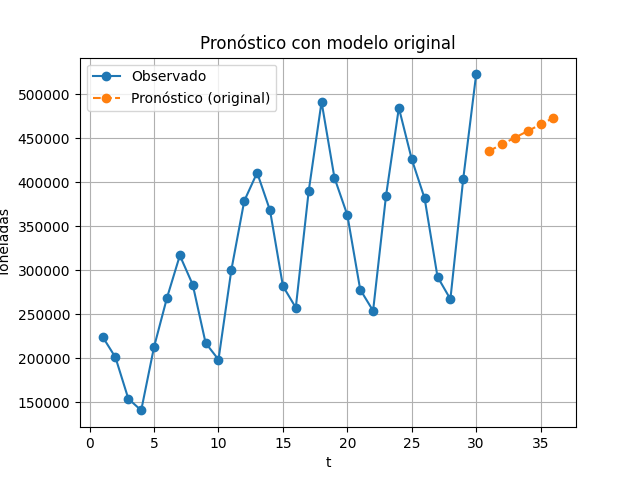
\includegraphics[width=0.7\linewidth]{../plots/python/avocado_exports_original_forecast.png}
          \caption{Pronóstico con modelo original (sin estacionalidad explícita).}
          \label{fig:forecast_original}
        \end{figure}
        \begin{figure}[H]
          \centering
          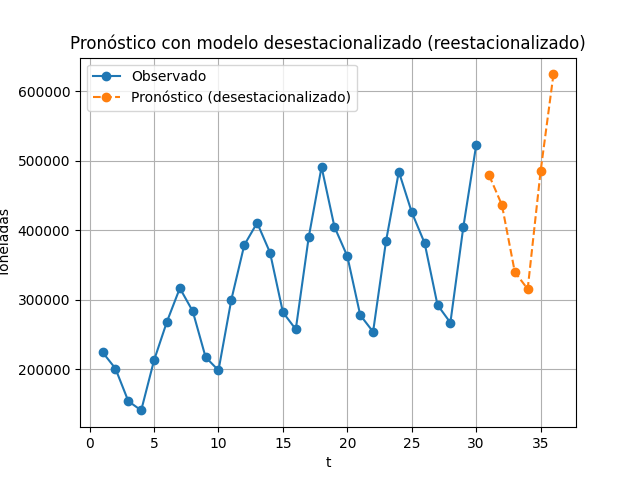
\includegraphics[width=0.7\linewidth]{../plots/python/avocado_exports_deseasonalized_forecast.png}
          \caption{Pronóstico con modelo desestacionalizado (reestacionalizado).}
          \label{fig:forecast_deseason}
        \end{figure}
        \noindent\textbf{Observaciones:}
        \begin{itemize}
          \item El \textbf{modelo original} proyecta valores entre \(\sim\!435\text{K}\) y \(\sim\!473\text{K}\) toneladas para 2024-bim1 al 6, con crecimiento suave y bandas relativamente estrechas, coherente con una tendencia lineal.
          \item El \textbf{modelo desestacionalizado} reproduce el patrón estacional: mínimos en bimestres 3--4 (\(\sim\!340\)K y \(\sim\!315\)K) y máximo en bimestre 6 (\(\sim\!624\)K), en línea con los índices estacionales ($I_6>1$ e $I_{3,4}<1$). Sus bandas son más amplias en los picos al reintroducir la estacionalidad.
        \end{itemize}
      }
    \end{enumerate}
%%%%%%%%%%%%%%%%%%%%%%%%%%%%%%%%%%%%%%%%%%%%%%%%%%%%%%%%%%%%%%%%%%%%%%%%%%%%%%%%%%%%%%%%%%%%%%%%%%%%%%%%%%%%%%%%%%%%%%%%%%%%%%%%%%%%%%%%%%%%%%%%%%%%%%%%%%%%%%%%%%%%%%%%%%%%%%%%%%%%%%%%%%%%%%
%%%%%%%%%%%%%%%%%%%%%%%%%%%%%%%%%%%%%%%%%%%%%%%%%%%%%%%%%%%%%%%%%%%%%%%%%%%%%%%%%%%%%%%%%%%%%%%%%%%%%%%%%%%%%%%%%%%%%%%%%%%%%%%%%%%%%%%%%%%%%%%%%%%%%%%%%%%%%%%%%%%%%%%%%%%%%%%%%%%%%%%%%%%%%%
\section{Link al repositorio con código fuente}
\href{https://github.com/enriquegomeztagle/MCD-Econometria/tree/main/HWs/TimeSeriesDeseasonalization}{https://github.com/enriquegomeztagle/MCD-Econometria/tree/main/HWs/TimeSeriesDeseasonalization}
%%%%%%%%%%%%%%%%%%%%%%%%%%%%%%%%%%%%%%%%%%%%%%%%%%%%%%%%%%%%%%%%%%%%%%%%%%%%%%%%%%%%%%%%%%%%%%%%%%%%%%%%%%%%%%%%%%%%%%%%%%%%%%%%%%%%%%%%%%%%%%%%%%%%%%%%%%%%%%%%%%%%%%%%%%%%%%%%%%%%%%%%%%%%%%
%%%%%%%%%%%%%%%%%%%%%%%%%%%%%%%%%%%%%%%%%%%%%%%%%%%%%%%%%%%%%%%%%%%%%%%%%%%%%%%%%%%%%%%%%%%%%%%%%%%%%%%%%%%%%%%%%%%%%%%%%%%%%%%%%%%%%%%%%%%%%%%%%%%%%%%%%%%%%%%%%%%%%%%%%%%%%%%%%%%%%%%%%%%%%%
\end{document}
%%%%%%%%%%%%%%%%%%%%%%%%%%%%%%%%%%%%%%%%%%%%%%%%%%%%%%%%%%%%%%%%%%%%%%%%%%%%%%%%%%%%%%%%%%%%%%%%%%%%%%%%%%%%%%%%%%%%%%%%%%%%%%%%%%%%%%%%%%%%%%%%%%%%%%%%%%%%%%%%%%%%%%%%%%%%%%%%%%%%%%%%%%%%%%
